%%%%
\documentclass[a4paper,11pt]{article}
%%%%
%%%%
%PACKAGES______________________________________________________________________________________
\usepackage{simplewick} %Allows Wick Notation
\usepackage{slashed} %Allows feynman slash notation 
\usepackage{graphicx} % graphics, pictures, figures
\usepackage{caption}
\usepackage{subcaption}
\usepackage{verbatim} % importing numerical scripts
\usepackage{multicol, float} % placing floats in right places
\usepackage{algpseudocode} % no idea...
\usepackage[utf8]{inputenc}
\usepackage{amssymb} %needed if not using mathdesign
\usepackage{amsmath}
\usepackage[OT1]{fontenc}
\usepackage{lmodern} %gfsartemisia, times, boisik, et cetera
\usepackage{braket} %dirac notation
\usepackage[cm]{fullpage} % for fulpage style
\usepackage{bm} % boldface vectors
\usepackage{float} % placing floats
\usepackage{relsize} % for \mathlarger command
\usepackage{mathrsfs} %?
\usepackage{textgreek} % cb-greek class
\usepackage{sectsty} % for centering sections
\usepackage{textcomp } % for nr. symbol
\usepackage[usenames, dvipsnames]{color} % defining own colors
\usepackage{type1cm} % scalable fonts
\usepackage{lettrine} % larger first letter in paragraph.
\usepackage{listings}
\usepackage{background} % used for top page text
%\usepackage{niceframe} % for old-school double frame
\usepackage{tikz} % figure config/ creation
%\usepackage{bbold}
%\usepackage{swrule} % for fancy line
%\usepackage{pdfpages} % for importing pdf

%%%%
%%%% SET-UP NEEDED FOR FURTHER PACKAGES
%%%%
\definecolor{hyperclrblue}{RGB}{30,90,125} %Definind own color ; blue
\definecolor{hyperclrorng}{RGB}{210,100,45}%Definind own color
\definecolor{hyperclrgreen}{RGB}{60,120,20}%Definind own color
\usepackage[colorlinks = true,
linkcolor = hyperclrblue,
urlcolor = blue,
citecolor = blue,
anchorcolor = blue]{hyperref} % link package
\usepackage{pgfplots} % to plot directly into latex
\pgfplotsset{compat=1.5} % needed forpgfplots
\usepackage{framed, color} % for framing/shaded box
\definecolor{shadecolor}{cmyk}{0,0,0.185,0} % color for shaded box
\usepackage{fancybox}
\usepackage[sc]{titlesec} % title package
%_______________________________________________________________________________________________
%NEW COMMANDS_________________________________________________________________________________
%\renewcommand*{\thefootnote}{$\dagger$} % creating dagger footnote
\newcommand*{\boisik}{\fontfamily{bsk}\selectfont} % change font to boisik command
\newcommand{\wf}{\text{\textpsi}} % defining wavefunctions as cbgreek class.
\newcommand{\bwf}{\text{\textPsi}} % defining Wavefunctions as cbgreek class.
\newcommand{\Q}{\hat{\text{\boisik Q}}} % defining operator-style 'Q'
\newcommand{\nlm}{\ket{n\ell m_\ell}} % defining wavefunctions as cbgreek class.
\newcommand{\nlmz}{\ket{n\ell m_\ell;0}} % defining wavefunctions as cbgreek class.
\newcommand{\nlmt}{\ket{n\ell m_\ell;t}} % defining wavefunctions as cbgreek class.
%_____________________________________________
%\numberwithin{equation}{section} %equations labeled by section
\sectionfont{\centering} % centering sections with 'sectsty'
\subsectionfont{\centering} % centering sections with 'sectsty'
\definecolor{myclr}{RGB}{190,90,20} %Definind own color
\renewcommand{\thesection}{\Roman{section}.} % Roman numerals for sections
\renewcommand{\thesubsection}{\Alph{subsection}} % Roman numerals for subsections
\titleformat{\section}{\large\scshape\centering}{\thesection}{1em}{} % Change the look of the section titles
\titleformat{\subsection}{\normalsize\centering\bfseries}{\thesubsection.}{1em}{} % Change the look of the section titles
\setlength{\columnsep}{0.7cm}
%______________________________________________________________________________________________
%%%%
%%%%_________________________________________________________________________________________
\begin{document}
%%%% TOP PAGE TEXT
{\SetBgContents{ \textit{{\small\textsc{ Ask J. Markestad, Thorbjørn V. Larsen Universitetet i Oslo. \hspace{3.5cm} \textit{\today}}}}}
\SetBgScale{1}
\SetBgColor{black}
\SetBgAngle{0}
\SetBgOpacity{1}
\SetBgPosition{current page.north east}
\SetBgVshift{-1.2cm}
\SetBgHshift{-10.5cm}
%%%% CREATING TITLE HEADER
$$\:$$
\begin{center}
	\vspace{0.2cm}%\boisik
	\fontsize{15}{15}\selectfont \textsc{ Project 3: Differential equations and the solar system},\\
	%{in}}\\
	\fontsize{13}{13}\selectfont \textsc{Fys $\textnormal{{4150}}$ }\\
	\vspace{0.4cm}
	\fontsize{12}{12}\selectfont {\textsc{ Ask J. Markestad, Thorbjørn V. Larsen }}\\
	\vspace{0.5cm}
\end{center}
%%%%
%%%%
%______________________________________________________________________________________________
%%%%
%%%%
	
%\includegraphics[scale = 0.48]{line}
\rule{\textwidth}{0.3pt}\par
		
%---------------------------------------------------------------------------------------------------------------------------------------
\begin{abstract}
	In this paper we discuss the basic ideas behind numerical solutions to ordinary differential equations, and their limitations by applying two well known methods; the forward Euler and velocity Verlet methods, to the many-body problem of our solar system. We then use these methods to do some numerical experiments, namely escape velocity of earth from the sun, and testing a general relativity correction to the Newtonian gravitational force.
\end{abstract}



		
\section*{Introduction}

Solving differential equations is one of the core problems that physicists encounter. It is therefore important to have a proper understanding of how to solve them, and since most cannot be solved analytically, numerical methods are a necessity in a physicists toolbox. We will briefly introduce two methods for solving ordinary differential equations; the forward Euler and velocity Verlet methods. We will then talk about their uses and limitations, conservation of energy and stability. To learn their applications we will use them to model our solar system and then use our model to do some numerical experiments. We will figure our the escape velocity of earth from the sun by running though a range of initial velocities. We will then look at a correction to the Newtonian gravitational force from General Relativity and test its validity by comparing our experiment to the observed perihelion precession of Mercury's orbit. 





\section*{Theory and Algorithms}

We will state the forward Euler and velocity Verlet methods, discuss their properties, and look at the solar system in more detail in this section. For a detailed derivation of these methods see Computational Physics Lecture Notes Fall 2015 \cite{M.Hjort-Jensen_CompFys} by Morten Hjort-Jensen.\\

The forward Euler method can be thought of geometrically. If you have an initial point, then you can find the next point by estimating the derivative in the initial point and using this gradient as the path to travel from the initial point to the next one by moving along it for a standard distance/step length. 

\begin{equation}
y_{i+1} = y_i + h y^{(1)}_{i} + O(h^2), \: \: \: \: h = \frac{y_{final}-y_{initial}}{Number\: of\: steps}
\label{Euler}	
\end{equation}

\begin{equation*}
y^{(1)}_{i+1} = y^{(1)}_i + h y^{(2)}_i + O(h^2)
\end{equation*}

Here we have set up the forward Euler method for a second order differential equation. For a higher order differential equation one would have several equations each using the next one to estimate the gradient of that order to be used. This method has a local error of $O(h^2)$ but will wave a global error of $O(h)$ when it is applied $N$ times to find the complete solution. Further, the forward Euler method is unstable in that not all step lengths give a finite solution for a differential equations. In other words, for exact solutions that converge, the numerical solution diverges if the step length is not chosen with care. \\

The velocity Verlet method is like most of our methods based on Taylor expansions. However, unlike the forward Euler method we also expand $y^{(2)}(t+h) 0 v^{(1)}(t+h)$ and use it to get the relation $h v_i^{(2)} \approx v_{i+1}^{(1)} - v_i^{(1)}$. This allows us to go to a higher order in the Taylor expansion of $y$ and $v$.

\begin{equation}
y_{i+1} = y_i + h v_{i} + \frac{h^2}{2} v^{(1)}_{i} + O(h^3)	
\label{Verlet}
\end{equation}

\begin{equation*}
v_{i+1} = v_i + \frac{h}{2}\left(v_{i+1}^{(1)} - v_i^{(1)}\right)  + O(h^3)
\end{equation*}

Note that we need to know the acceleration for both the point we are at and for the next position to calculate the next velocity step, meaning we need to do the position calculation first. This method is also stable, i.e. for every step length the computed and exact solution will have the same characteristics, but will have a local error of $O(h^3)$ and the solution will have a global error of $O(h^2)$. Another characteristic of the velocity Verlet method is that is preserves energy, which we will explicitly test and compare with the forward Euler method. \\

Let us look more specifically at the solar system at hand. The system is described by Newtons law of gravitation and Newtons second law, which means we know the forces and thus the accelerations involved as functions of the position. The gravitational law for a two body system, f.eks. the sun earth system is given by:

\begin{equation}
F_G = \frac{G M_{sun} M_{earth}}{r^2}
\label{2bodygrav}
\end{equation}

Further we want to do a variable change into some more fitting units for simulating the solar system, namely astronomical units (1 AU = $1.5 \times 10^{11}$m), years and solar masses($M_{sun} = 2\times 10^{30} kg$). To achieve this we rescale using a circular orbit of 1 AU. Then, from Newtons second law:

\begin{equation}
v^2 r = G M_{sun} = 4 \pi^2 \frac{AU^3}{yr^2}
\label{circorbi}
\end{equation}

Where we used that the period for the orbit should be one year. This allows us to get rid of the $G M_{sun}$ factor in our calculations. We then divide the force by the mass of the moving object to find the acceleration and we can then apply the numerical methods previously mentioned. The next step is then to introduce more bodies into our calculations and thus taking us away for situations that are analytically solvable. Let us look are the inclusion of a third planet, Venus. Each body will now have a force acting on them that is the sum of the forces for each two body combination that they are a part of. So, the earth will have a force term that is identical with the previous earth sun term, but will also have a term:

\begin{equation}
F_G = \frac{G M_{venus} M_{earth}}{r_{earth-venus}^2}
\label{2bodygrav_ve}
\end{equation}

Again, we are interested in the acceleration that this provides earth with so we will dived by the earth mass here but we are now left with a $G M_{venus}$ factor. Here we multiply and divide by $M_{sun}$ so we can write $M_{venus}$ in terms of solar masses and we get the $G M_{sun}$ factor that we have rescaled to be $(2\pi)^2$. The forces for Venus will be similar but with the earth mass having to be rescaled. This leaves us with the coupled differential equations for earth in the x direction:

\begin{align}
& \frac{dx}{dt} = v(t)
& \frac{d v_x}{dt} = - \frac{(2\pi)^2 M_{venus}}{r_{earth-venus}^2} - \frac{(2\pi)^2 }{r_{earth-sun}^2}
\label{eqofmotion}
\end{align}

With similar equations for the y and z directions, and for Venus and the Sun. Adding more planets will then equate to adding more of these acceleration terms, and we can then add arbitrarily many bodies to our simulation.\\

The perihelion precession of Mercury's orbit has been known for a very long time, and was a known problem to Einstein when he developed General relativity, and it was the very first success of General Relativity that it predicted and explained Mercury's perihelion precession. We will attempt recreate this effect in our simulation by adding a correction term to the force, from General Relativity:

\begin{equation}
F_G = \frac{G M_{sun} M_{mercury}}{r_{sun-mercury}^2} \left[ 1 + \frac{3 l^2}{r_{sun-mercury}^2 c^2} \right]
\label{2bodygrav_GR}
\end{equation}

Where $l = |\vec{r}\times \vec{v}|$ is the magnitude of mercury's orbital angular momentum. We should note here that this correction will be very small given that c, the speed of light, is a very large number and it therefore only gives an effect for planets sufficiently close to each other, explaining why only Mercury observes this effect. We can measure the precession by checking the perihelion angle $\tan\left(\theta_p\right) = \frac{y_p}{x_p}$, which changes by an observed $43$ arcseconds per century.

\subsection*{Algorithms}
In this project we based the structure of the C++ program mostly on a already built class from the FYS4150 course. The implementation of the Euler method was already finished but as this method is inherently unstable with respect to energy conservation we implemented the Velocity Verlet method ourselves. In equation \ref{Verlet} we see that we generally have the following workflow(calling $a_i = v^{(1)}_i$)
\begin{lstlisting}
for all timesteps:
	for all bodies:
		x_(i+1) = f(a_i,x_i,v_i)
	for all bodies:
		a_i+1 = f'(x_i+1)
	for all bodies:
		v_(i+1)=f''(v_i, a_i+1, a_i)
	for all bodies:
		a_i = a_i+1
\end{lstlisting}
In the implementation of this we would save some flops by precalculating $h^2/2$ and $h/2$ giving
\begin{align}
	flops = \#(line1) +  \#(line2)+ \#(line3) = (4+ \# a_{i+1} + 3)*\#( bodies*timesteps) \\
	= (7 + \# (a_{i+1}))*\#( bodies)*N
\end{align}
%dette saa ikke pent ut
This seemingly looks like an expression that scales linearly both with the number of bodies and number of timesteps N, but and important contribution is hidden in the calculation of $a_{i+1}$ that dominates over 7 when the number of planets become large.  To calculate this expression we have to loop over all planets and then find the force from all other planets that exists in our system where such contributions are on the form of \ref{eqofmotion}. As the forces from two planets A and B are equal, but with opposite direction we can save 50$\%$ of the calculations by adding the acceleration to both planets we are looking at, and as we only look at planet pairs $(A,B)$ where $A\neq B$ we have 
\begin{align}
	\# a_{i+1}*bodies = (bodies-1)! *\#(a_{(A_i,B_j)})
\end{align}
We then continue to look at each such expression $F_{(A_i,B_j)}$
\begin{align}
F_{(A_i,B_j)}= -\frac{(2\pi)^2 M_j M_i}{r^2}
\end{align}
where we can precalculate the $4\pi^2$ factor, $r^2$ gives 5 flops and leads to the total of 8 flops. We sum over all such terms for each planet, and then divide by the mass of the planet. We see that for each such evaluation we have to multiply the masses of the planets, which is something that potentially could be precalculated as a matrix. This was not implemented as the effective limit in our simulations was the part of the program that wrote to a file(took 99\% of the CPU time for a 2 body system) so any further work in reducing flops was not done. However when we only only at the calculations they scale in general by using Stirlings approximation ($n! \propto \sqrt{n}n^n$) which is rather good giving
\begin{align}
	flops \propto N * (bodies)(bodies-1)^{bodies-1/2}
\end{align}
The time spent on the writing to files is not a specific part of the algorithm, but on a sidetrack we could potentially speed up the code by declaring a matrix for each planet to hold all the positions and velocities for each time-step and only at the end write to file. We speculate that this would have the advantage of a faster speed since we only have a workflow between the CPU and short term memory, while in the constant writing to file for each step would necessarily access the long term memory and such a process is inherently slower. On the other hand a disadvantage of such a way of saving the data would give some limitations on the number of planets and time steps as this stores all the data in the short term memory which is orders of magnitude smaller. In our implementation we chose to use the setup with writing in each step, as this already was implemented. 



\section*{Results}

We ran a simulation of a Earth-Sun system where the Sun starts at rest in the origin, with the Earth in a circular orbit at radius 1 AU \ref{circorbi} starting along the x-axis with initial velocity in the y-direction, for using both the forward Euler \ref{Euler} and velocity Verlet \ref{Verlet} methods. The simulation was run for a 100 year period with $10^{6}$ timesteps, and the results are shown in figure \ref{fig:verlet_vs_euler}. We see in subfigure \ref{fig:E_S_circular_euler} that for the forward Euler method we get an constantly increasing spiral orbit, arising from the error of the Euler method. While for the Verlet method, subfigure \ref{fig:E_S_circular_verlet}, We see a stable circular orbit over the same period.

\begin{figure}[H]
	\centering
	\begin{subfigure}[b]{1\textwidth}
		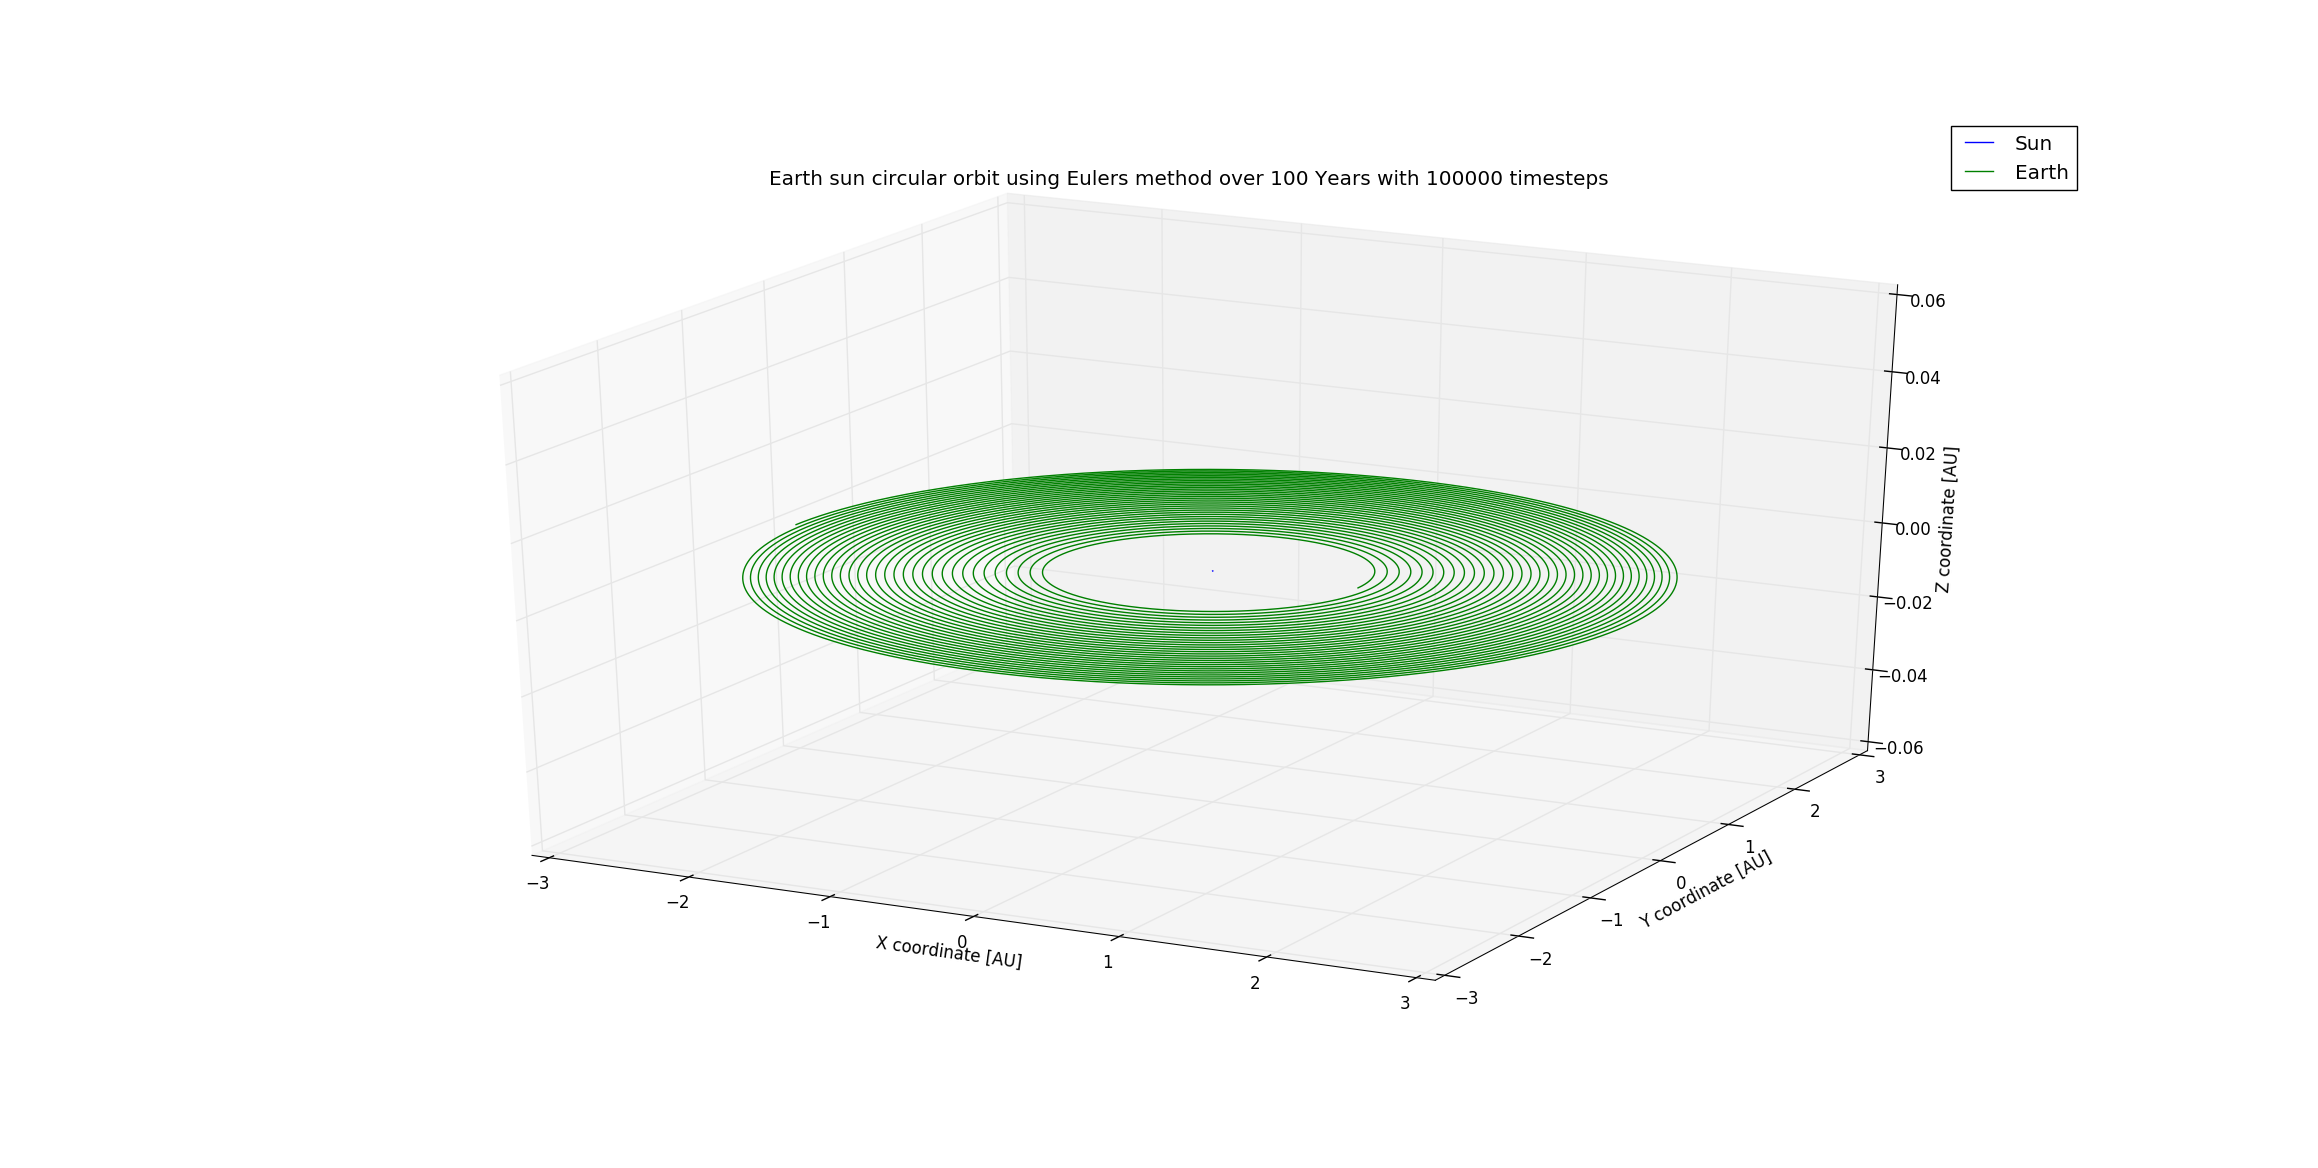
\includegraphics[scale=0.3]{figure_4}
		\caption{Earth-sun system with Sun initially at rest at origin and Earth at 1 AU in the x axis with circular orbit initial velocity. Calculated using the velocity Verlet method over 100 years with $10^{6}$ timesteps.}
		\label{fig:E_S_circular_verlet}
	\end{subfigure}
	\begin{subfigure}[b]{1\textwidth}
		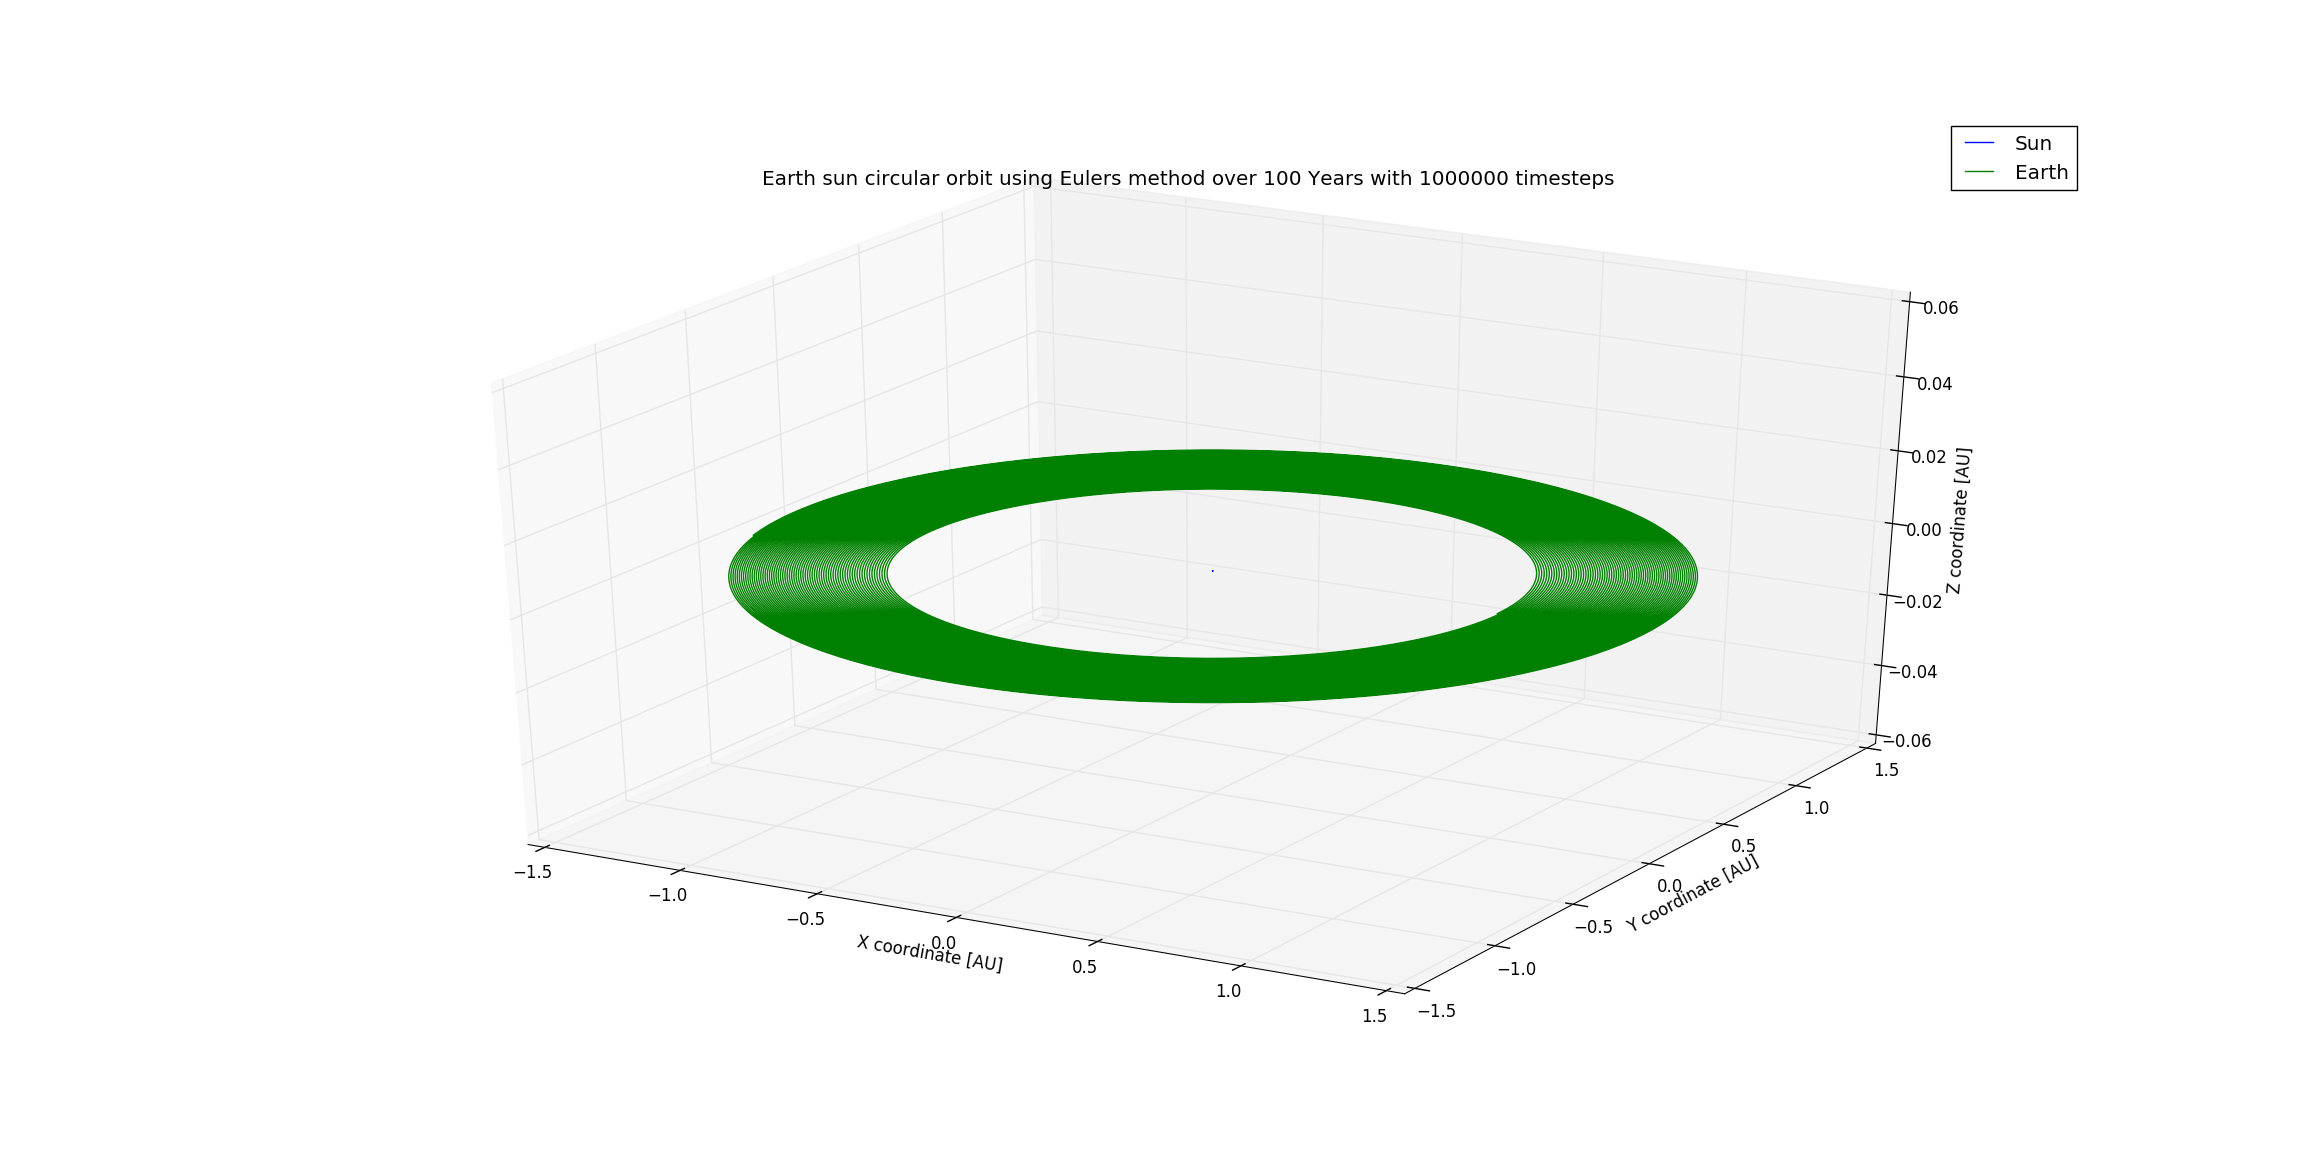
\includegraphics[scale=0.3]{figure_5}
		\caption{Earth-sun system with Sun initially at rest at origin and Earth at 1 AU in the x axis with circular orbit initial velocity. Calculated using the forward Euler method over 100 years with $10^{6}$ timesteps.}
		\label{fig:E_S_circular_euler}
	\end{subfigure}
	\caption{Comparison between the numerical simulations of Earth-Sun system for circular Earth orbit using the velocity Verlet method and the forward Euler method.}
	\label{fig:verlet_vs_euler}
\end{figure}

In these next figures \ref{fig:verlet_vs_euler_energies} we see the kinetic, potential and total energies of the same circular Earth-Sun system. Again we see the stability of the Verlet method fig \ref{fig:E_S_circular_verlet_energies} and the instability of the Euler method fig \ref{fig:E_S_circular_euler_energies}.

\begin{figure}[H]
	\centering
	\begin{subfigure}[b]{1\textwidth}
		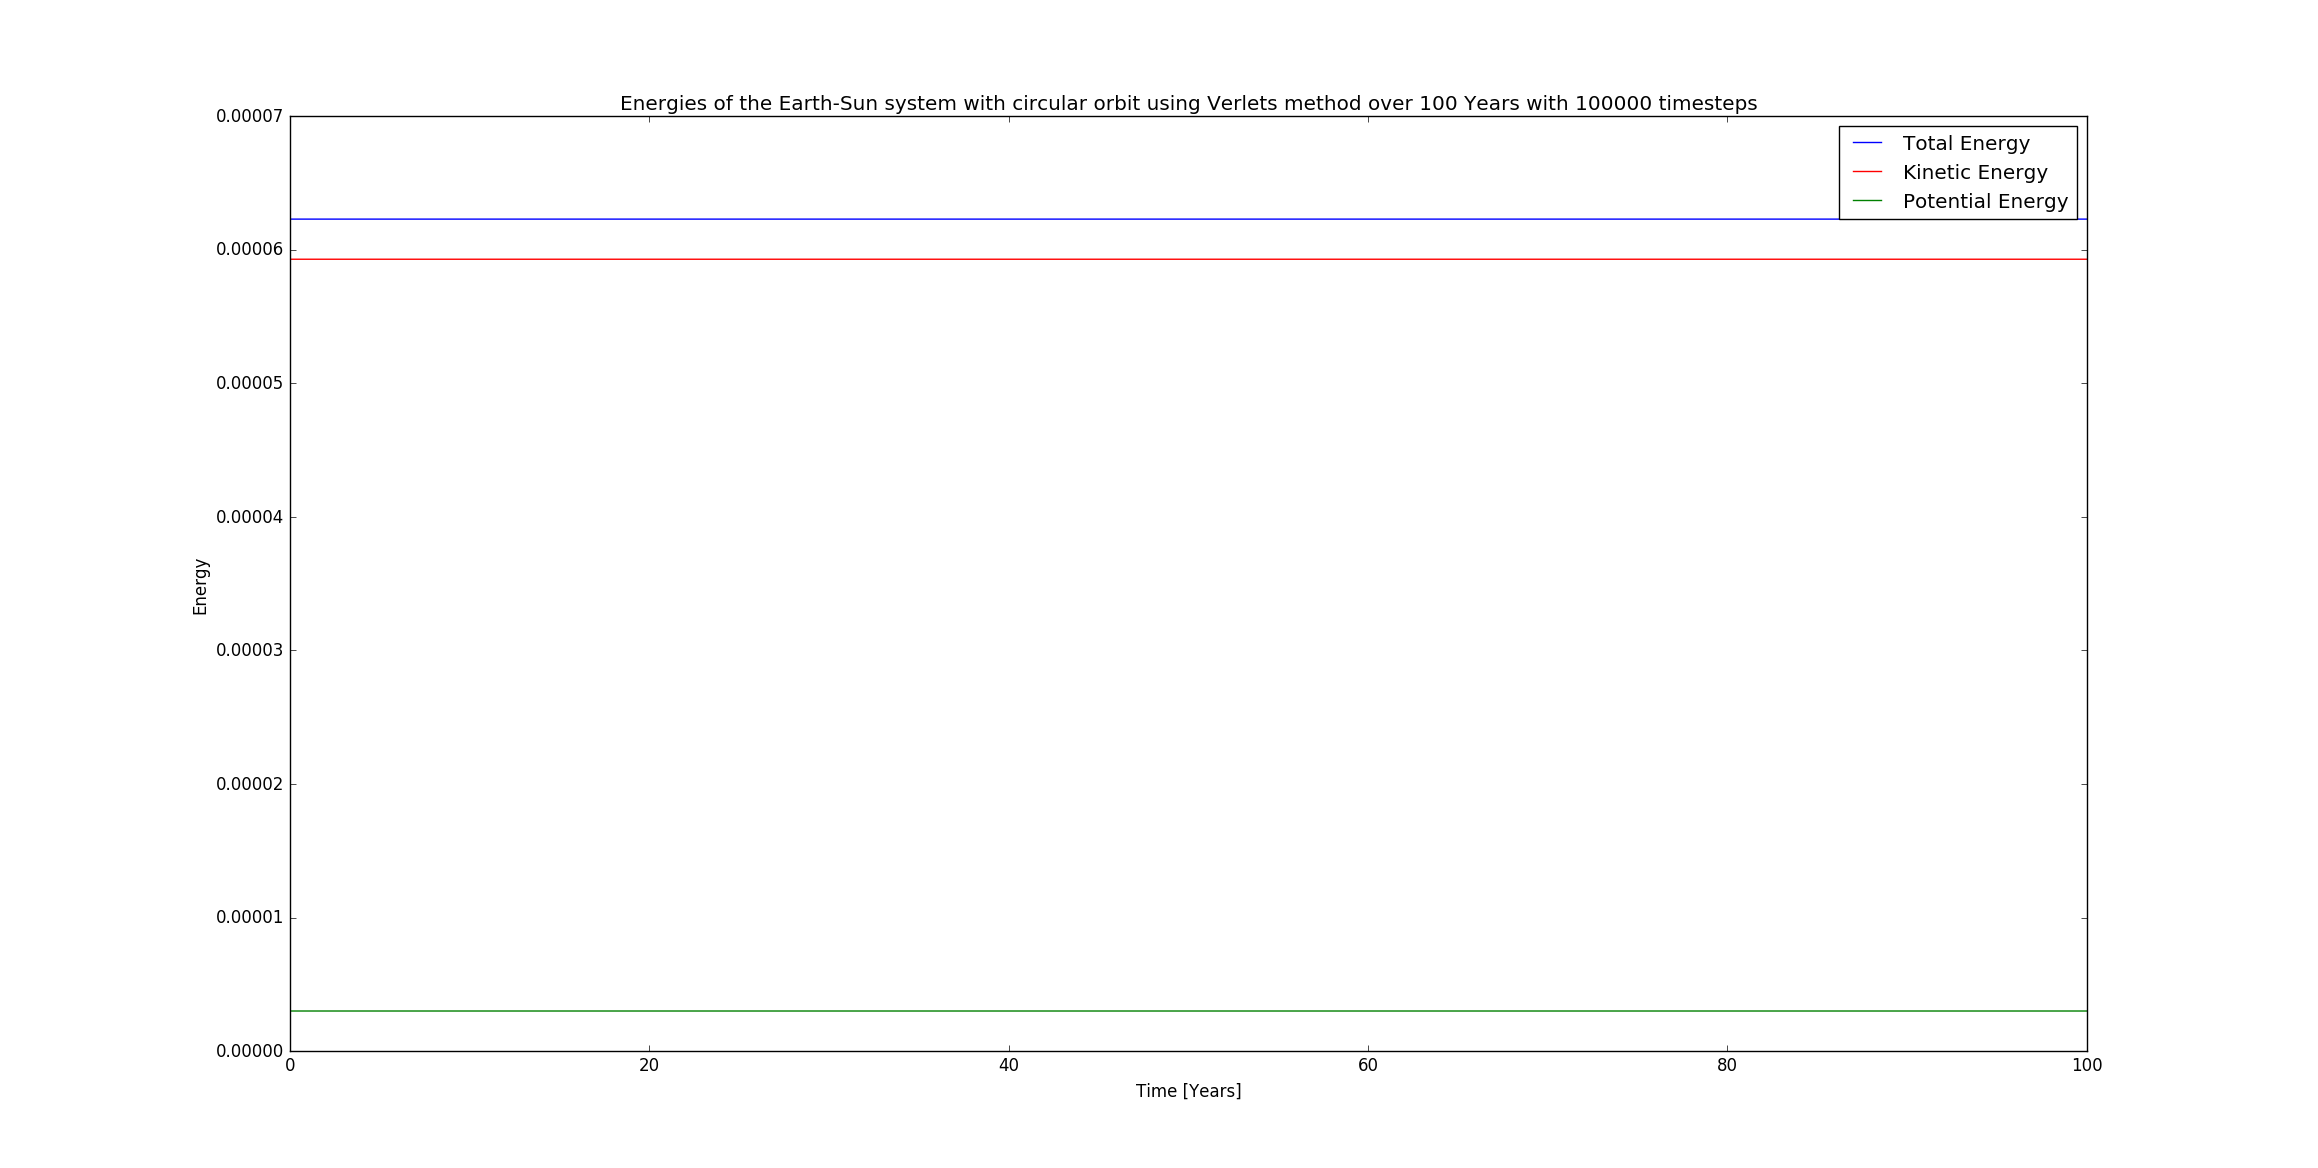
\includegraphics[scale=0.3]{figure_9}
		\caption{Energies of the Earth-sun system with Sun initially at rest at origin and Earth at 1 AU in the x axis with circular orbit initial velocity. Calculated using the velocity Verlet method over 100 years with $10^{6}$ timesteps.}
		\label{fig:E_S_circular_verlet_energies}
	\end{subfigure}
	\begin{subfigure}[b]{1\textwidth}
		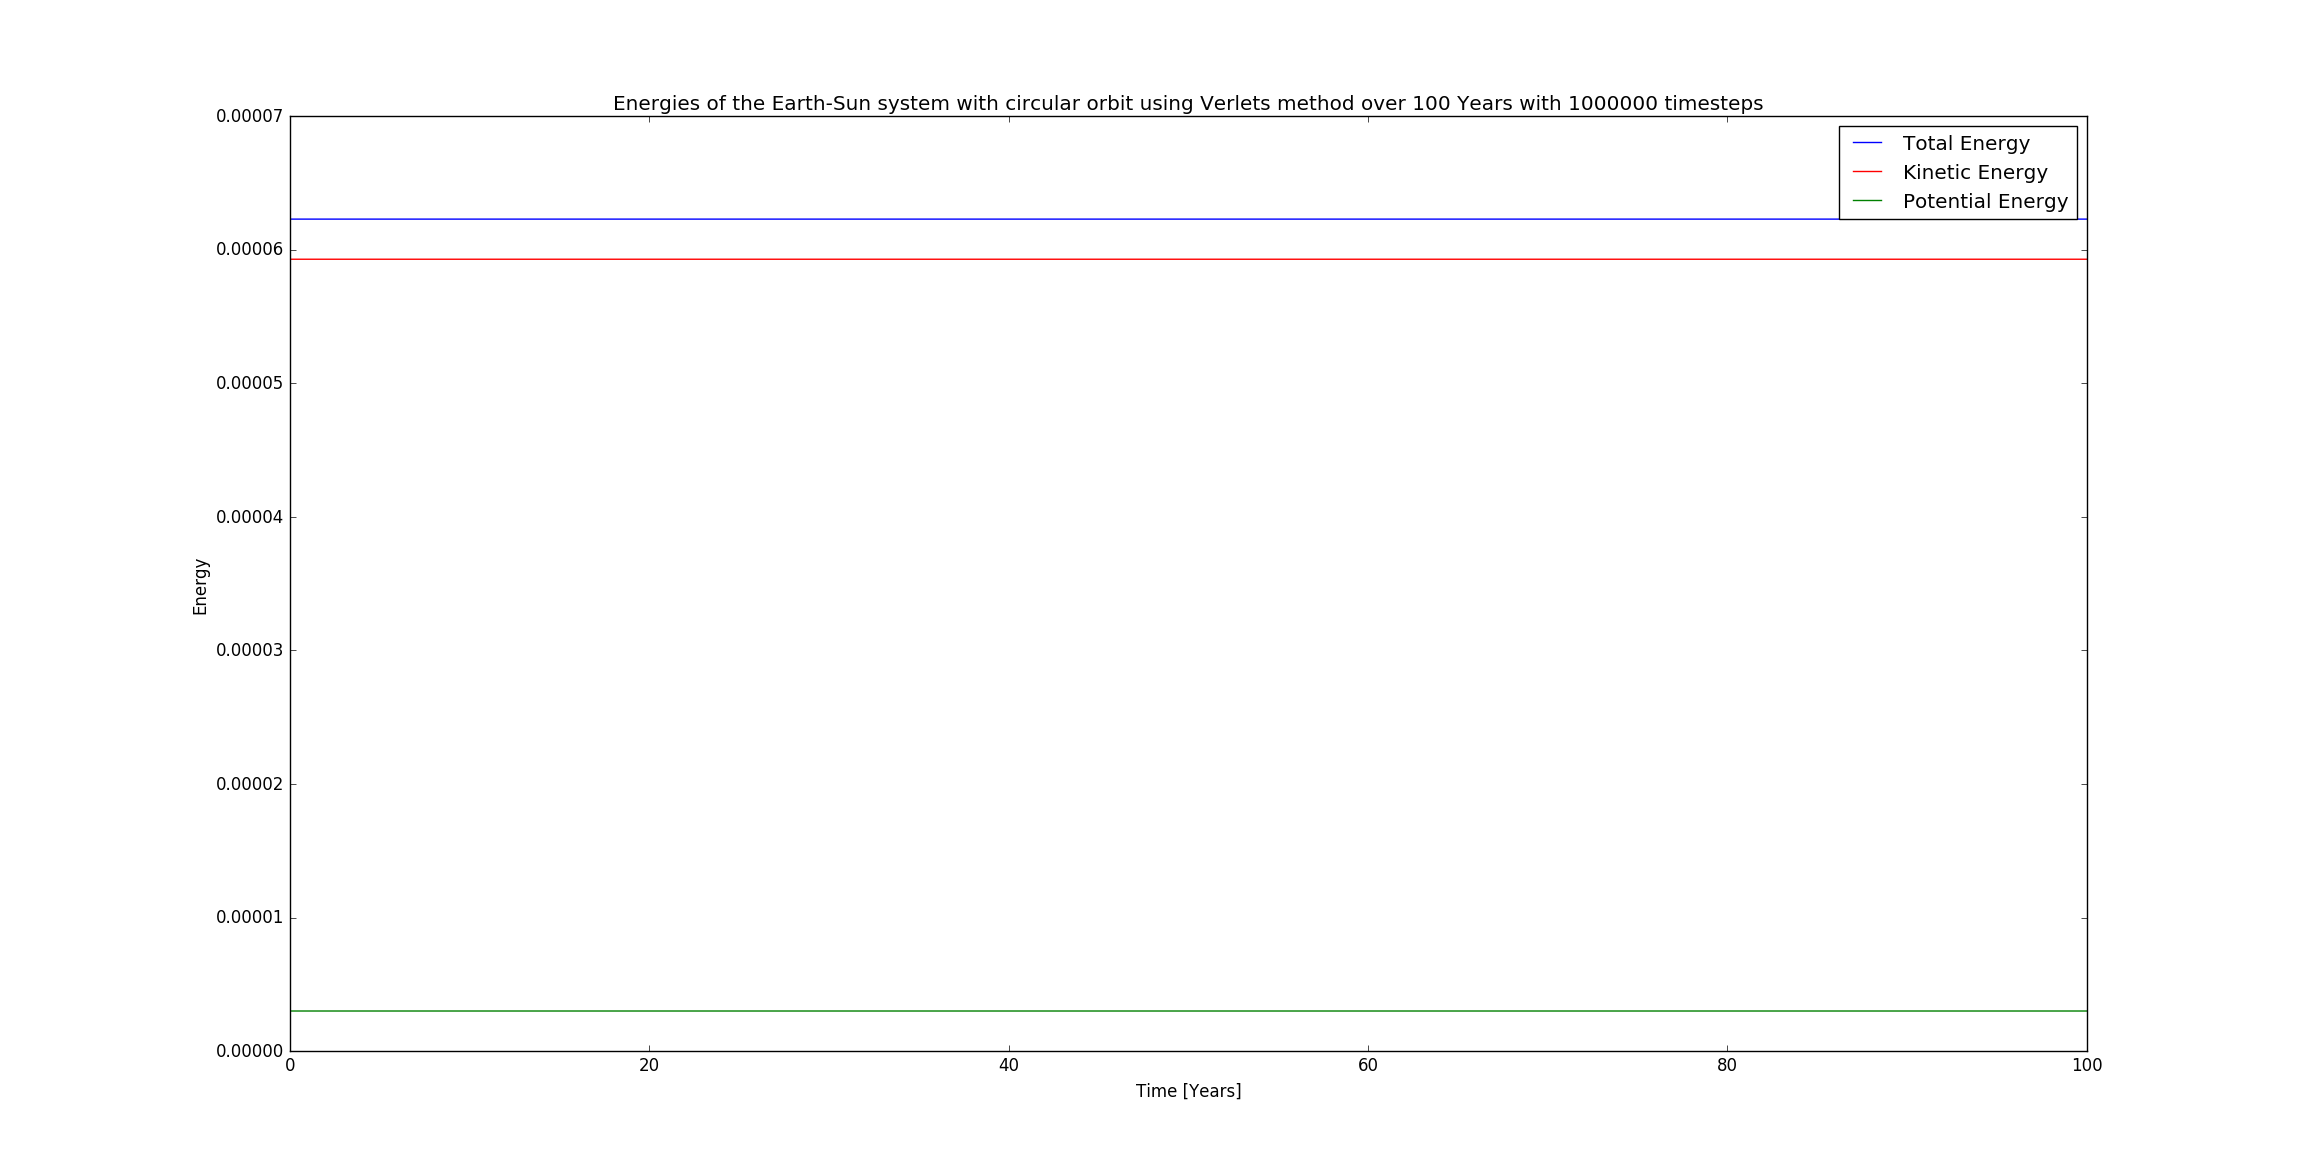
\includegraphics[scale=0.3]{figure_10}
		\caption{Energies of the Earth-sun system with Sun initially at rest at origin and Earth at 1 AU in the x axis with circular orbit initial velocity. Calculated using the forward Euler method over 100 years with $10^{6}$ timesteps.}
		\label{fig:E_S_circular_euler_energies}
	\end{subfigure}
	\caption{Comparison between the energies of the numerical simulations of Earth-Sun system for circular Earth orbit using the velocity Verlet method and the forward Euler method.}
	\label{fig:verlet_vs_euler_energies}
\end{figure}



Further, we wanted to find an estimate of the escape velocity of the Earth starting a 1 AU from the Sun. In figure \ref{fig:E_S_escape} we see two initial velocities which gives some very extreme elliptical orbit with respectively 8.76 AU/year and 8.833 AU/year initial velocities. We see however, fig \ref{fig:E_S_escape3}, that if we increase the initial velocity to 8.906 AU/year, escape is achieved.


\begin{figure}[H]
	\centering
	\begin{subfigure}[b]{1\textwidth}
		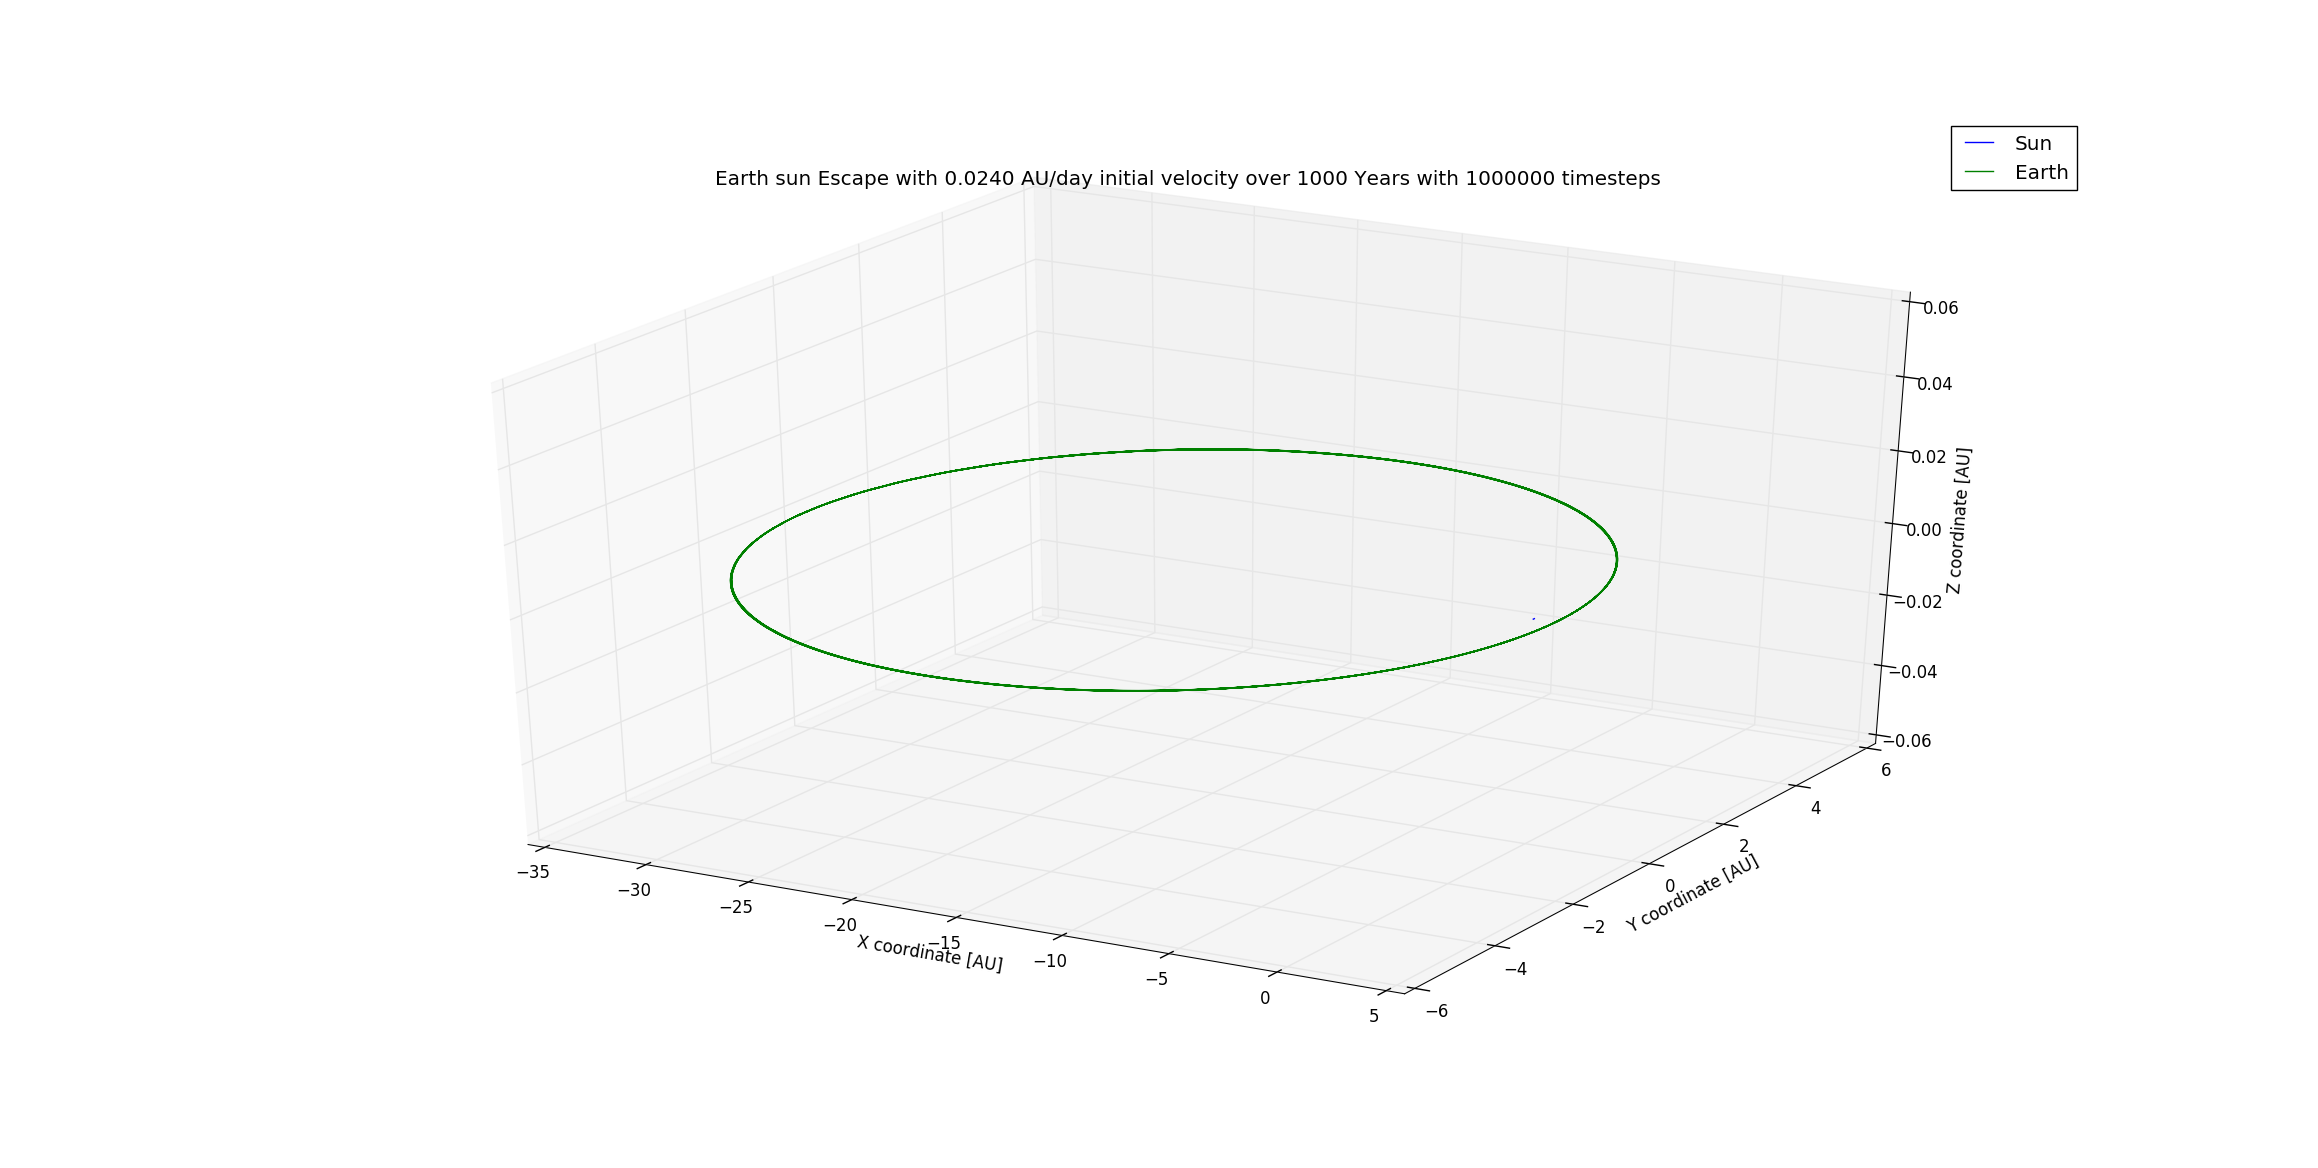
\includegraphics[scale=0.3]{figure_6}
		\caption{Earth-sun system with Sun initially at rest at origin and Earth at 1 AU in the x axis with 0.0240 AU/day or 8.76 AU/year initial velocity in the y direction. Calculated using the velocity Verlet method over 1000 years with $10^{6}$ timesteps. Notice the very elliptical orbit with y direction only varying with ~12 AU in the orbit while x varies with ~40 AU.}
		\label{fig:E_S_escape1}
	\end{subfigure}
	\begin{subfigure}[b]{1\textwidth}
		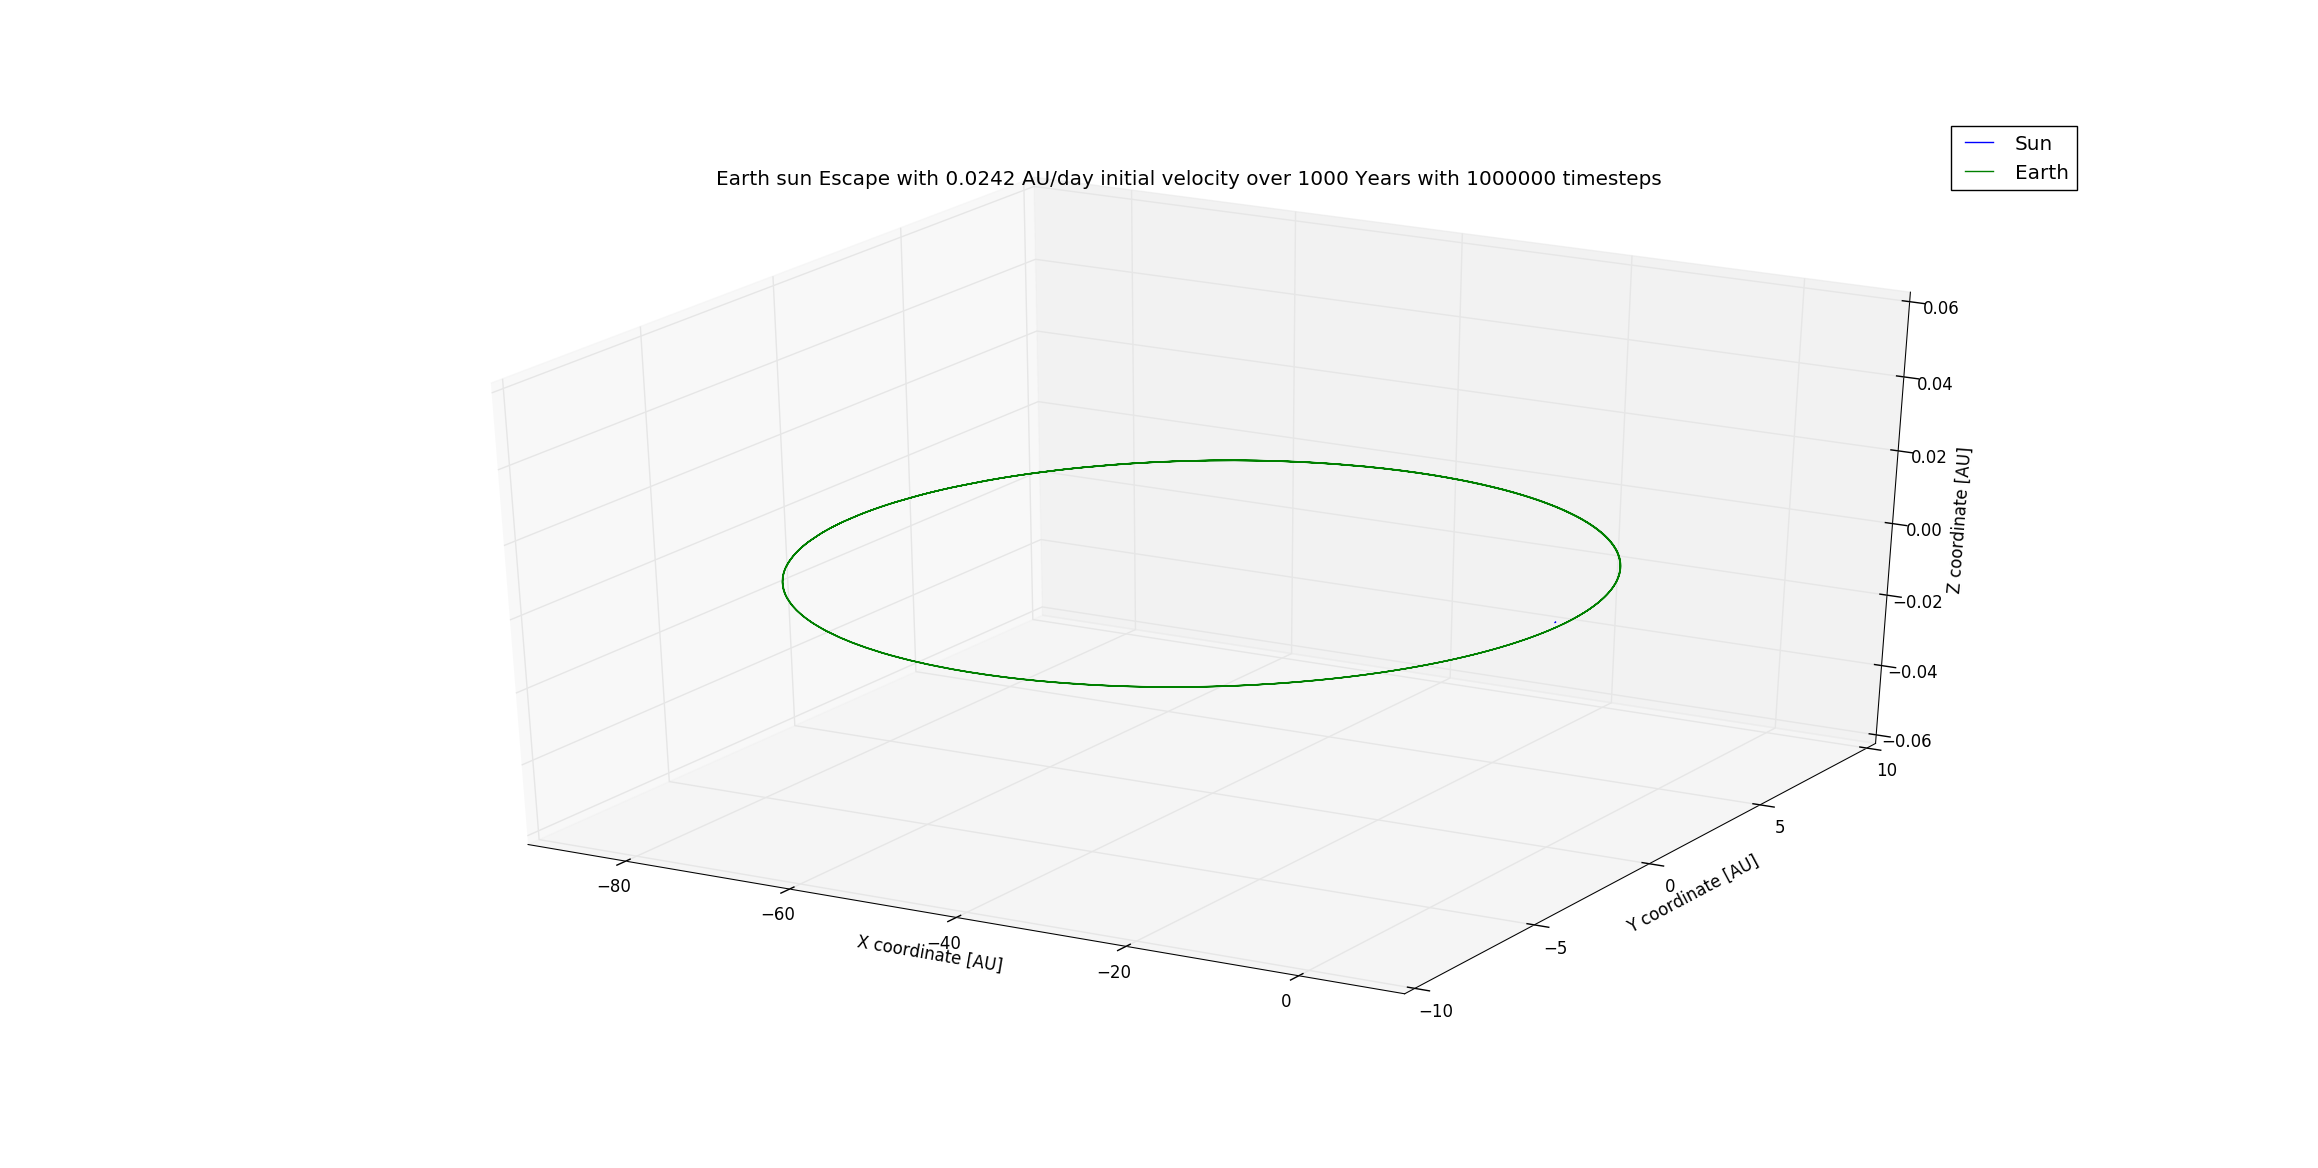
\includegraphics[scale=0.3]{figure_7}
		\caption{Earth-sun system with Sun initially at rest at origin and Earth at 1 AU in the x axis with 0.0242 AU/day or 8.833 AU/year initial velocity in the y direction. Calculated using the velocity Verlet method over 1000 years with $10^{6}$ timesteps.Notice the very elliptical orbit with y direction only varying with ~20 AU in the orbit while x varies with ~80 AU.}
		\label{fig:E_S_escape2}
	\end{subfigure}
	\caption{Comparison between Earth-Sun orbits with different initial velocities.}
	\label{fig:E_S_escape}
\end{figure}

\begin{figure}[H]
	\centering
	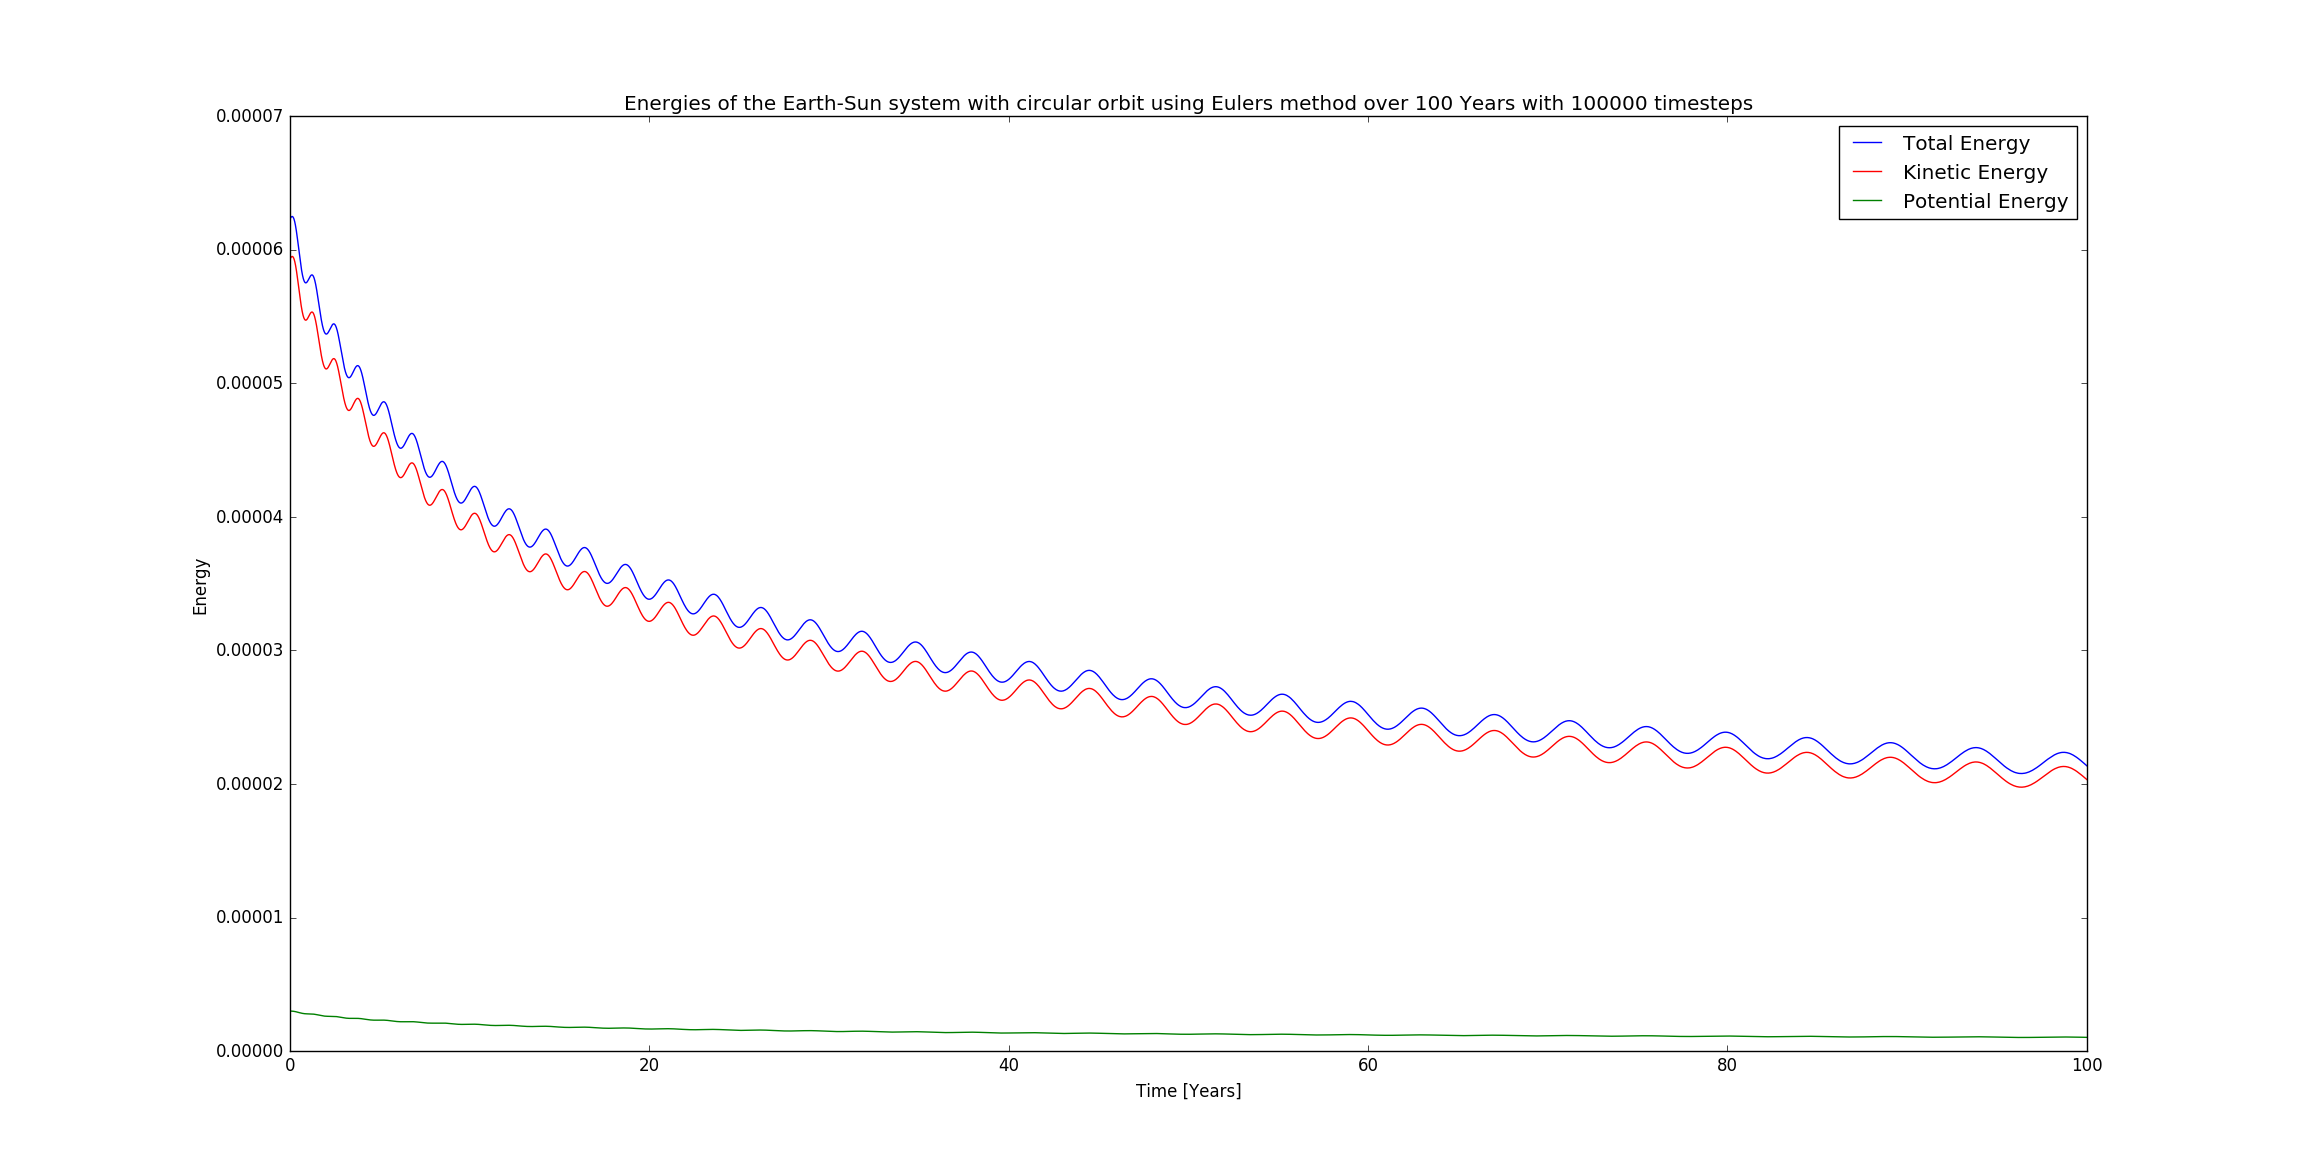
\includegraphics[scale=0.35]{figure_8}
	\caption{Earth-sun system with Sun initially at rest at origin and Earth at 1 AU in the x axis with 0.0243 AU/day or 8.906 AU/year initial velocity in the y direction. Calculated using the velocity Verlet method over 1000 years with $10^{6}$ timesteps. Here we see that we have achieved escape velocity.}
	\label{fig:E_S_escape3}
\end{figure}


From figure \ref{fig:verlet_vs_euler} we have seen the accuracy and stability of the velocity Verlet method, so we use it to simulate our Solar system, including Pluto. We ran the simulation for a period of 300 years to get the complete Pluto orbit, using $10^{6}$ timesteps. The result is seen in figure \ref{fig:solar_system}. We can't quite see the orbits of the innermost planets in this figure, but if we could we would see some very strange behavior for Mercury.



\begin{figure}[H]
	\centering
	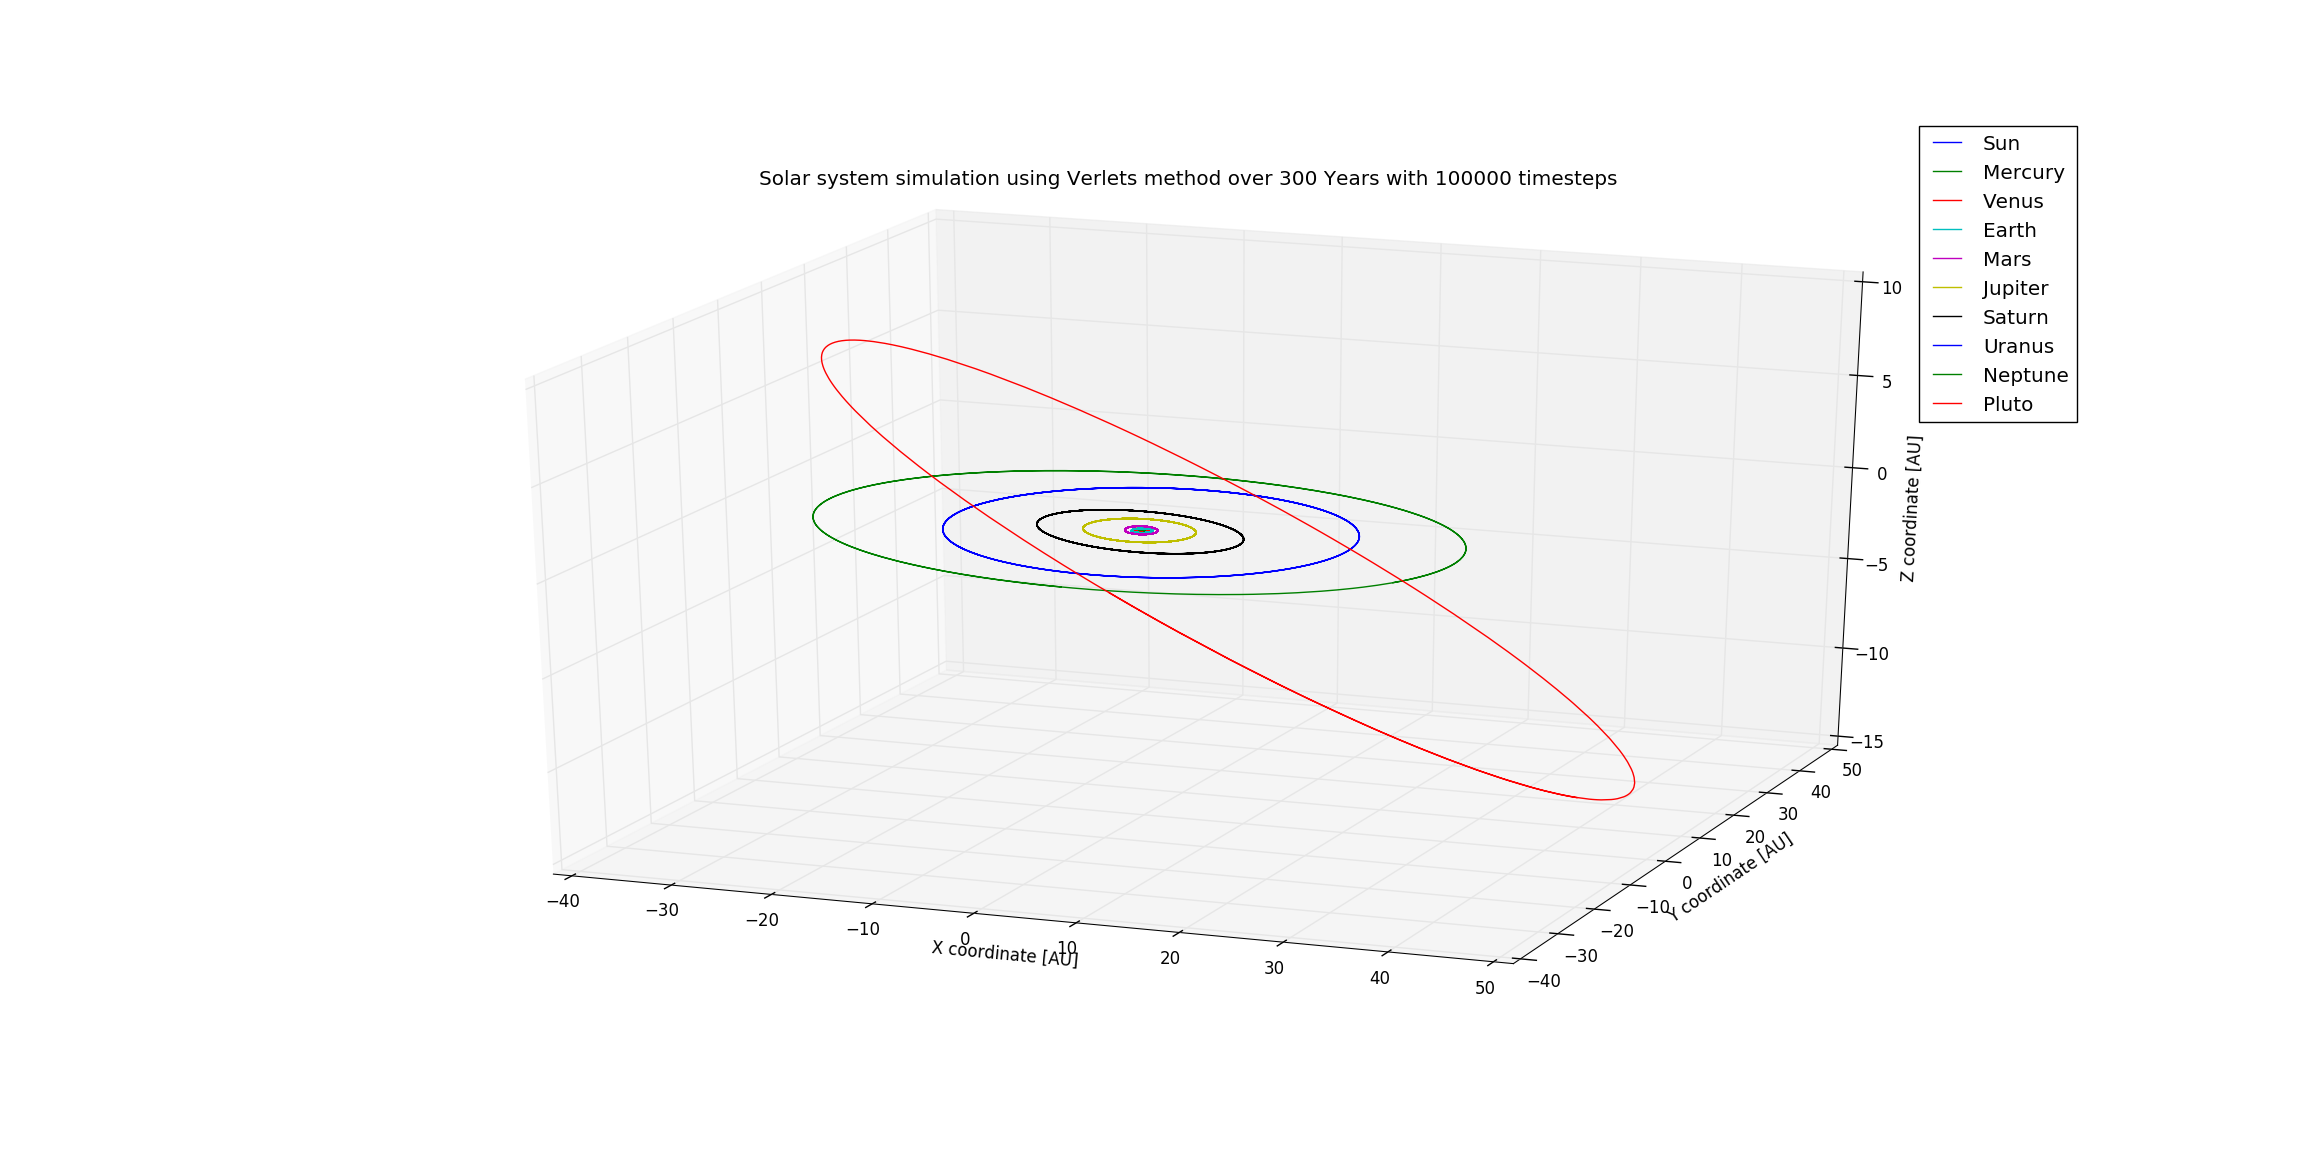
\includegraphics[scale=0.35]{figure_1}
	\caption{Simulation of the Solar system using the Verlet method with all the planets, including Pluto, for 300 years to get Pluto's entire orbit with $10^{6}$ timesteps.}
	\label{fig:solar_system}
\end{figure}

Since Mercury passes so close to the Sun it achieves some very large velocities, which gives errors when using the Verlet method when the timestep is too large. For the "small" number of timesteps $10^{6}$ that we have used previously we observe something that looks like an extreme perihelion precession over the 100 year time period, when we know that precession should be almost unobservable. So to get the correct behavior we increase the number of timesteps to 10 billion. Calculating the perihelion angle and plotting it in arc seconds vs. time we get figure \ref{fig:perihelion}.


\begin{figure}[H]
	\centering
	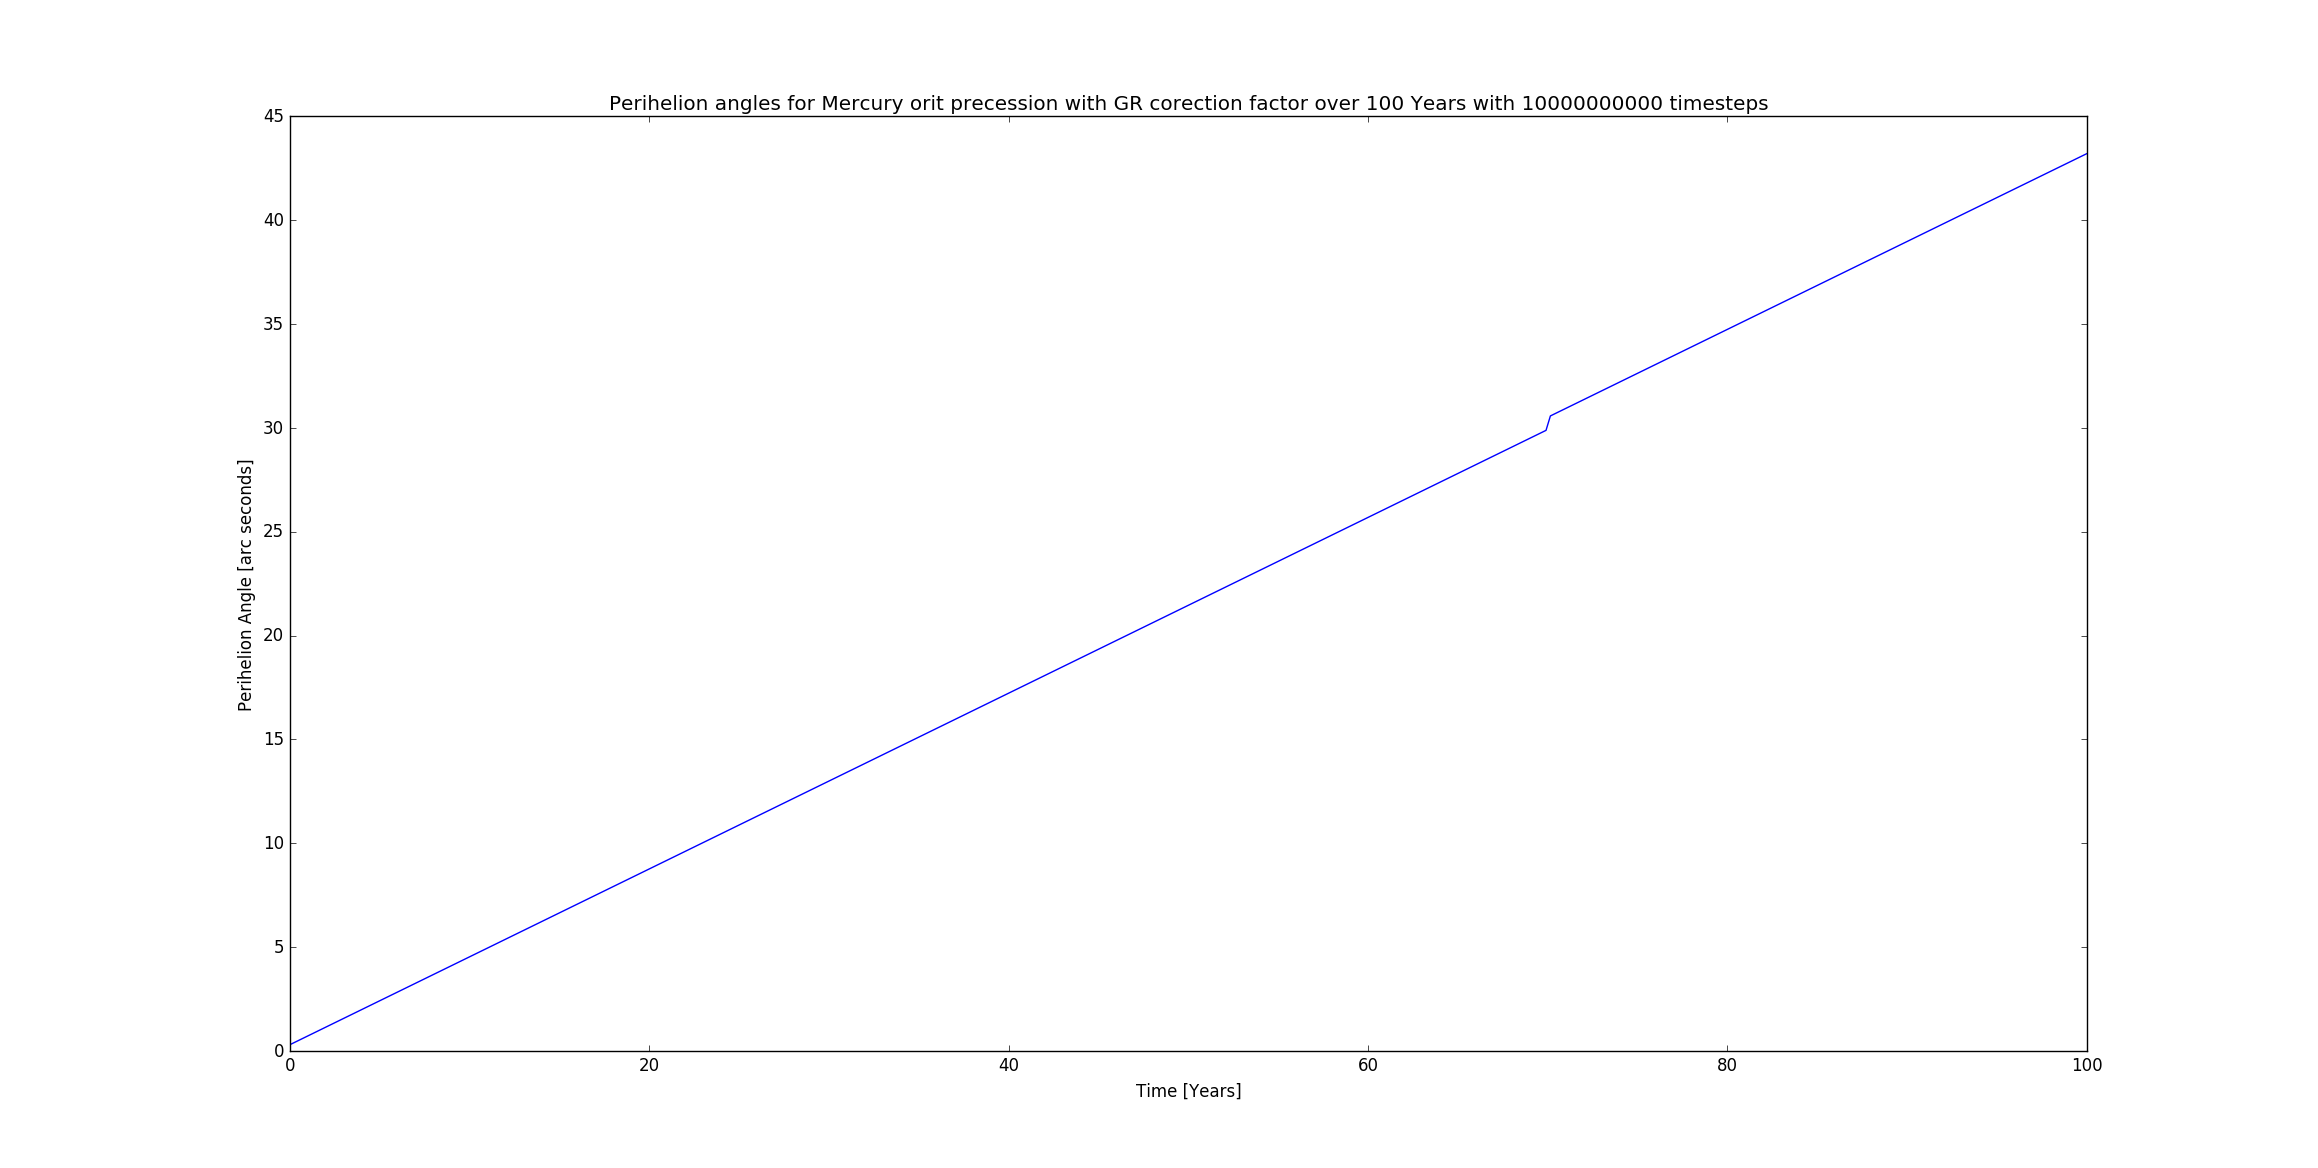
\includegraphics[scale=0.35]{figure_2}
	\caption{The Perihelion angle in arc seconds over a century for the Sun-Mercury system where we have included the GR correction factor in the force for this calculation, see eq. \ref{2bodygrav_GR}. From our theory we would expect this plot to be a straight line, however we see a small kink that emerges from a lack of timesteps. These result were calculated with $10^{10}$ timesteps, with less timesteps we saw more kinks and when we increased to $10^{11}$ we started getting more kinks again and the final angle had a larger error compared to the actual perihelion angle after a century.}
	\label{fig:perihelion}
\end{figure}

Observe the little kink in the plot in figure \ref{fig:perihelion}. From the theory we would expect this line to be straight, and this little kink is an indication that we still don't have a large enough number of time steps, as we see more kinks for less timesteps. However when we increase the number of timesteps by a factor of 10 we run into greater inaccuracies from loss of numerical precision. We would therefore need a different, more accurate method if we want to improve the results for Mercury. The final perihelion angle, after a century, was $43.196$ arc seconds.


\section*{Conclusion}






\begin{thebibliography}{3}
			
	\bibitem{M.Hjort-Jensen_CompFys}
	Morten Hjort-Jensen
	\emph{ Computational Physics Lecture Notes Fall 2015}
	Department of Physics, University of Oslo
	2015
	\url{https://github.com/CompPhysics/ComputationalPhysics/blob/master/doc/Lectures/lectures2015.pdf}
	
	
			
			
			
			
\end{thebibliography}
		
		
		
		
		
		
		
		
		
%__________________________________________________________________________
\end{document}